\begin{figure}[!htbp]
  \centering
  \begin{subfigure}[b]{0.25\textwidth}
    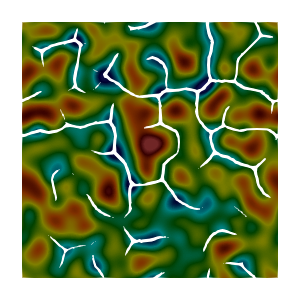
\includegraphics[width=\textwidth]{Chapter4/figures/2D/Gc_sqexp_cartesian_5_5_rho_0_seed_a_with_crack_140.png}
    \caption{$\mathcal{D}^* = 3.06$}
    \label{fig: Chapter4/2D/Gc_sqexp_cartesian_5_5_rho_0_seed_a_with_crack_140}
  \end{subfigure}
  \begin{subfigure}[b]{0.25\textwidth}
    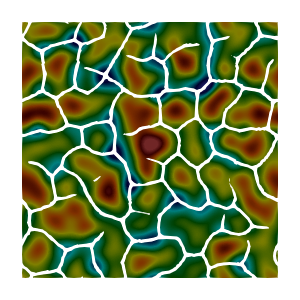
\includegraphics[width=\textwidth]{Chapter4/figures/2D/Gc_sqexp_cartesian_5_5_rho_0_seed_a_with_crack_160.png}
    \caption{$\mathcal{D}^* = 3.76$}
    \label{fig: Chapter4/2D/Gc_sqexp_cartesian_5_5_rho_0_seed_a_with_crack_160}
  \end{subfigure}
  \begin{subfigure}[b]{0.25\textwidth}
    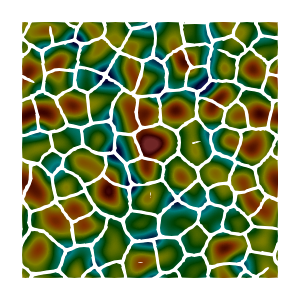
\includegraphics[width=\textwidth]{Chapter4/figures/2D/Gc_sqexp_cartesian_5_5_rho_0_seed_a_with_crack_220.png}
    \caption{$\mathcal{D}^* = 5.17$}
    \label{fig: Chapter4/2D/Gc_sqexp_cartesian_5_5_rho_0_seed_a_with_crack_220}
  \end{subfigure}
  \begin{subfigure}[b]{0.08\textwidth}
    \caption*{$\Gc^*$}
    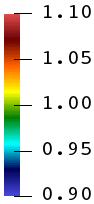
\includegraphics[width=\textwidth]{Chapter4/figures/rainbow_vertical.png}
    \vspace{0.15in}
  \end{subfigure}

  \begin{subfigure}[b]{0.25\textwidth}
    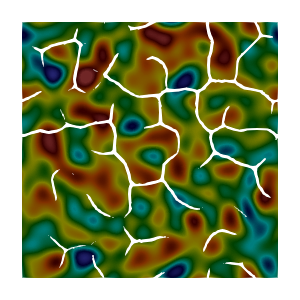
\includegraphics[width=\textwidth]{Chapter4/figures/2D/psic_sqexp_cartesian_5_5_rho_0_seed_a_with_crack_140.png}
    \caption{$\mathcal{D}^* = 3.06$}
    \label{fig: Chapter4/2D/psic_sqexp_cartesian_5_5_rho_0_seed_a_with_crack_140}
  \end{subfigure}
  \begin{subfigure}[b]{0.25\textwidth}
    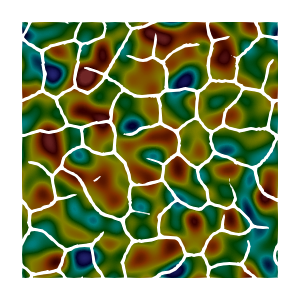
\includegraphics[width=\textwidth]{Chapter4/figures/2D/psic_sqexp_cartesian_5_5_rho_0_seed_a_with_crack_160.png}
    \caption{$\mathcal{D}^* = 3.76$}
    \label{fig: Chapter4/2D/psic_sqexp_cartesian_5_5_rho_0_seed_a_with_crack_160}
  \end{subfigure}
  \begin{subfigure}[b]{0.25\textwidth}
    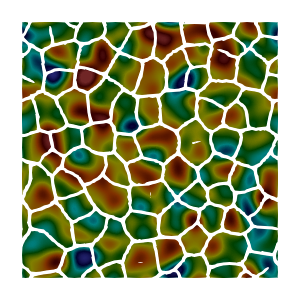
\includegraphics[width=\textwidth]{Chapter4/figures/2D/psic_sqexp_cartesian_5_5_rho_0_seed_a_with_crack_220.png}
    \caption{$\mathcal{D}^* = 5.17$}
    \label{fig: Chapter4/2D/psic_sqexp_cartesian_5_5_rho_0_seed_a_with_crack_220}
  \end{subfigure}
  \begin{subfigure}[b]{0.08\textwidth}
    \caption*{$\psi_c^*$}
    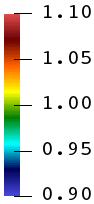
\includegraphics[width=\textwidth]{Chapter4/figures/rainbow_vertical.png}
    \vspace{0.15in}
  \end{subfigure}
  \caption{Snapshots of phase field at different loading levels with $d \geqslant 0.75$ plotted over (a-c) fracture toughness $\Gc$ and (d-f) critical fracture energy $\psi_c$ with an underlying PSE covariance function }
  \label{fig: Chapter4/2D/compare_sensitivity_sqexp}
\end{figure}

\begin{figure}[!htbp]
  \centering
  \begin{subfigure}[b]{0.25\textwidth}
    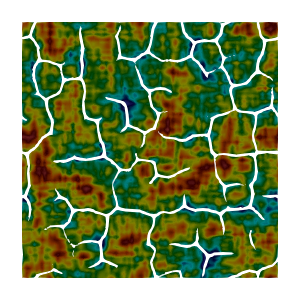
\includegraphics[width=\textwidth]{Chapter4/figures/2D/Gc_exp_cartesian_5_5_rho_0_seed_b_with_crack_140.png}
    \caption{$\mathcal{D}^* = 3.06$}
    \label{fig: Chapter4/2D/Gc_exp_cartesian_5_5_rho_0_seed_a_with_crack_140}
  \end{subfigure}
  \begin{subfigure}[b]{0.25\textwidth}
    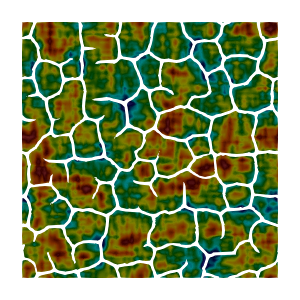
\includegraphics[width=\textwidth]{Chapter4/figures/2D/Gc_exp_cartesian_5_5_rho_0_seed_b_with_crack_160.png}
    \caption{$\mathcal{D}^* = 3.76$}
    \label{fig: Chapter4/2D/Gc_exp_cartesian_5_5_rho_0_seed_a_with_crack_160}
  \end{subfigure}
  \begin{subfigure}[b]{0.25\textwidth}
    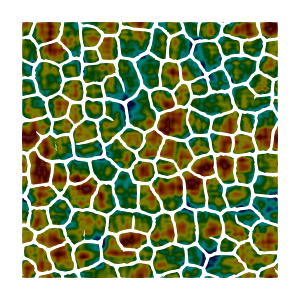
\includegraphics[width=\textwidth]{Chapter4/figures/2D/Gc_exp_cartesian_5_5_rho_0_seed_b_with_crack_220.png}
    \caption{$\mathcal{D}^* = 5.17$}
    \label{fig: Chapter4/2D/Gc_exp_cartesian_5_5_rho_0_seed_a_with_crack_220}
  \end{subfigure}
  \begin{subfigure}[b]{0.08\textwidth}
    \caption*{$\Gc^*$}
    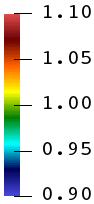
\includegraphics[width=\textwidth]{Chapter4/figures/rainbow_vertical.png}
    \vspace{0.15in}
  \end{subfigure}

  \begin{subfigure}[b]{0.25\textwidth}
    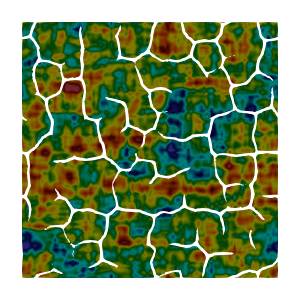
\includegraphics[width=\textwidth]{Chapter4/figures/2D/psic_exp_cartesian_5_5_rho_0_seed_b_with_crack_140.png}
    \caption{$\mathcal{D}^* = 3.06$}
    \label{fig: Chapter4/2D/psic_exp_cartesian_5_5_rho_0_seed_a_with_crack_140}
  \end{subfigure}
  \begin{subfigure}[b]{0.25\textwidth}
    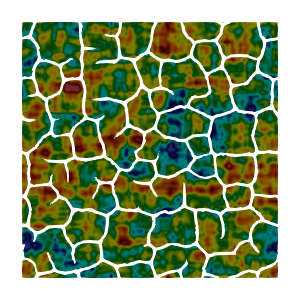
\includegraphics[width=\textwidth]{Chapter4/figures/2D/psic_exp_cartesian_5_5_rho_0_seed_b_with_crack_160.png}
    \caption{$\mathcal{D}^* = 3.76$}
    \label{fig: Chapter4/2D/psic_exp_cartesian_5_5_rho_0_seed_a_with_crack_160}
  \end{subfigure}
  \begin{subfigure}[b]{0.25\textwidth}
    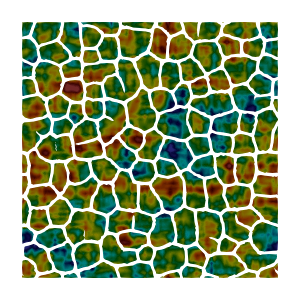
\includegraphics[width=\textwidth]{Chapter4/figures/2D/psic_exp_cartesian_5_5_rho_0_seed_b_with_crack_220.png}
    \caption{$\mathcal{D}^* = 5.17$}
    \label{fig: Chapter4/2D/psic_exp_cartesian_5_5_rho_0_seed_a_with_crack_220}
  \end{subfigure}
  \begin{subfigure}[b]{0.08\textwidth}
    \caption*{$\psi_c^*$}
    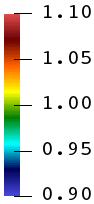
\includegraphics[width=\textwidth]{Chapter4/figures/rainbow_vertical.png}
    \vspace{0.15in}
  \end{subfigure}
  \caption{Snapshots of phase field at different loading levels with $d \geqslant 0.75$ plotted over (a-c) fracture toughness $\Gc$ and (d-f) critical fracture energy $\psi_c$ with an underlying PE covariance function }
  \label{fig: Chapter4/2D/compare_sensitivity_exp}
\end{figure}
